\documentclass{article}

% \usepackage[latin1]{inputenc}
\usepackage[french]{babel}
\usepackage[T1]{fontenc}

\usepackage{lastpage}
\usepackage{fancyhdr}
\usepackage{graphicx}
\usepackage{pdflscape}

\usepackage[a4paper, margin=2.2cm, footskip=12.3pt]{geometry}

\setcounter{secnumdepth}{0}

\newcommand{\header} {
    \setlength{\headheight}{30pt}\pagestyle{fancy}
    \fancyhead[L]{
\includegraphics[height=20pt]{../logo.pdf}}\fancyhead[C]{}
    \fancyhead[R]{Vitória Cosmo, Aubry Mangold, Eva Ray\\\today}\fancyfoot[C]{}
    \fancyfoot[R]{Page \thepage~sur \pageref{LastPage}}\renewcommand{\footrulewidth}{0.3pt}
}

\newcommand{\ul}{\underline}
\newcommand{\ttt}{\texttt}

\title{Gestion d'un service de réparation d'objets\\[1ex]Modélisation relationnelle}
\author{Vitória Cosmo, Aubry Mangold, Eva Ray}
\date{DATE}

\begin{document}
\header


\maketitle

\section{Conversion EA-relationnel}

\begin{itemize}
    \item \ttt{person (\ul{person\_id}, phone\_no, name, comment)}
    \subitem \ttt{name} \ttt{NOT NULL}
    \subitem \ttt{phone\_no} \ttt{UNIQUE}

    \item \ttt{customer (\ul{customer\_id}, tos\_accepted, private\_note)}
    \subitem \ttt{customer\_id} référence \ttt{person.id}
    \subitem \ttt{tos\_accepted} \ttt{NOT NULL}

    \item \ttt{collaborator (\ul{collaborator\_id}, email)}
    \subitem \ttt{collaborator\_id} référence \ttt{Person.id}
    \subitem \ttt{email} \ttt{NOT NULL}

    \item \ttt{manager (\ul{manager\_id})}
    \subitem \ttt{manager\_id} référence \ttt{collaborator.id} 

    \item \ttt{technician (\ul{technician\_id})}
    \subitem \ttt{technician\_id} référence \ttt{collaborator.id}

    \item \ttt{receptionist (\ul{receptionist\_id})}
    \subitem \ttt{receptionist\_id} référence \ttt{collaborator.id}

    \item \ttt{language (\ul{name})}

    \item \ttt{receptionist\_language (\ul{id}, \ul{language\_id})}
    \subitem \ttt{id} référence \ttt{receptionist.receptionist\_id}
    \subitem \ttt{language\_id} référence \ttt{language.name}

    \item \ttt{specialization (\ul{name})}
    
    \item \ttt{technician\_specialization (\ul{technician\_id}, \ul{spec\_id})}
    \subitem \ttt{technician\_id} référence \ttt{technician.technician\_id}
    \subitem \ttt{spec\_id} référence \ttt{specialization.name}

    \item \ttt{Reparation (\ul{id}, object\_id, customer\_id, receptionist\_id, date\_created, date\_modified, quote, description, estimated\_duration, reparation\_state, quote\_state)}
    
    \subitem \ttt{date\_created}, \ttt{description}, \ttt{reparation\_state}, \ttt{quote\_state} \ttt{NOT NULL}
    \subitem \ttt{object\_id} référence \ttt{object.object\_id} \ttt{UNIQUE, NOT NULL}
    \subitem \ttt{customer\_id} référence \ttt{customer.customer\_id} \ttt{NOT NULL}
    \subitem \ttt{receptionist\_id} référence \ttt{receptionist.receptionist\_id} \ttt{NOT NULL}

    \item \ttt{technician\_reparation (\ul{technician\_id}, \ul{reparation\_id})}
    \subitem \ttt{technician\_id} référence \ttt{technician.technician\_id} 
    \subitem \ttt{reparation\_id} référence \ttt{reparation.reparation\_id}

    \item \ttt{specialization\_reparation (\ul{spec\_id}, \ul{reparation\_id})}
    \subitem \ttt{spec\_id} référence \ttt{specialization.name}
    \subitem \ttt{reparation\_id} référence \ttt{reparation.id}

    \item \ttt{sms (\ul{id}, reparation\_id, date\_created, message, sender, receiver, processing\_state)}
    \subitem \ttt{reparation\_id} référence \ttt{reparation.reparation\_id} \ttt{NOT NULL}

    \item \ttt{object (\ul{object\_id}, customer\_id, name, fault\_desc, location, remark, serial\_no, brand, category)}
    \subitem \ttt{name}, \ttt{fault\_desc}, \ttt{location}, \ttt{brand}, \ttt{category} \ttt{NOT NULL}
    \subitem \ttt{customer\_id} référence \ttt{customer.id} \ttt{NOT NULL}

    \item \ttt{brand (\ul{name})}
    \item \ttt{category (\ul{name})}
    \item \ttt{sale (\ul{object\_id}, \ul{id\_sale}, price, date\_created, date\_sold)}
    \subitem \ttt{object\_id} référence \ttt{object.id}

\end{itemize}


\pagebreak
% \begin{landscape}
% \begin{figure}[!htb]
%         \centering
%         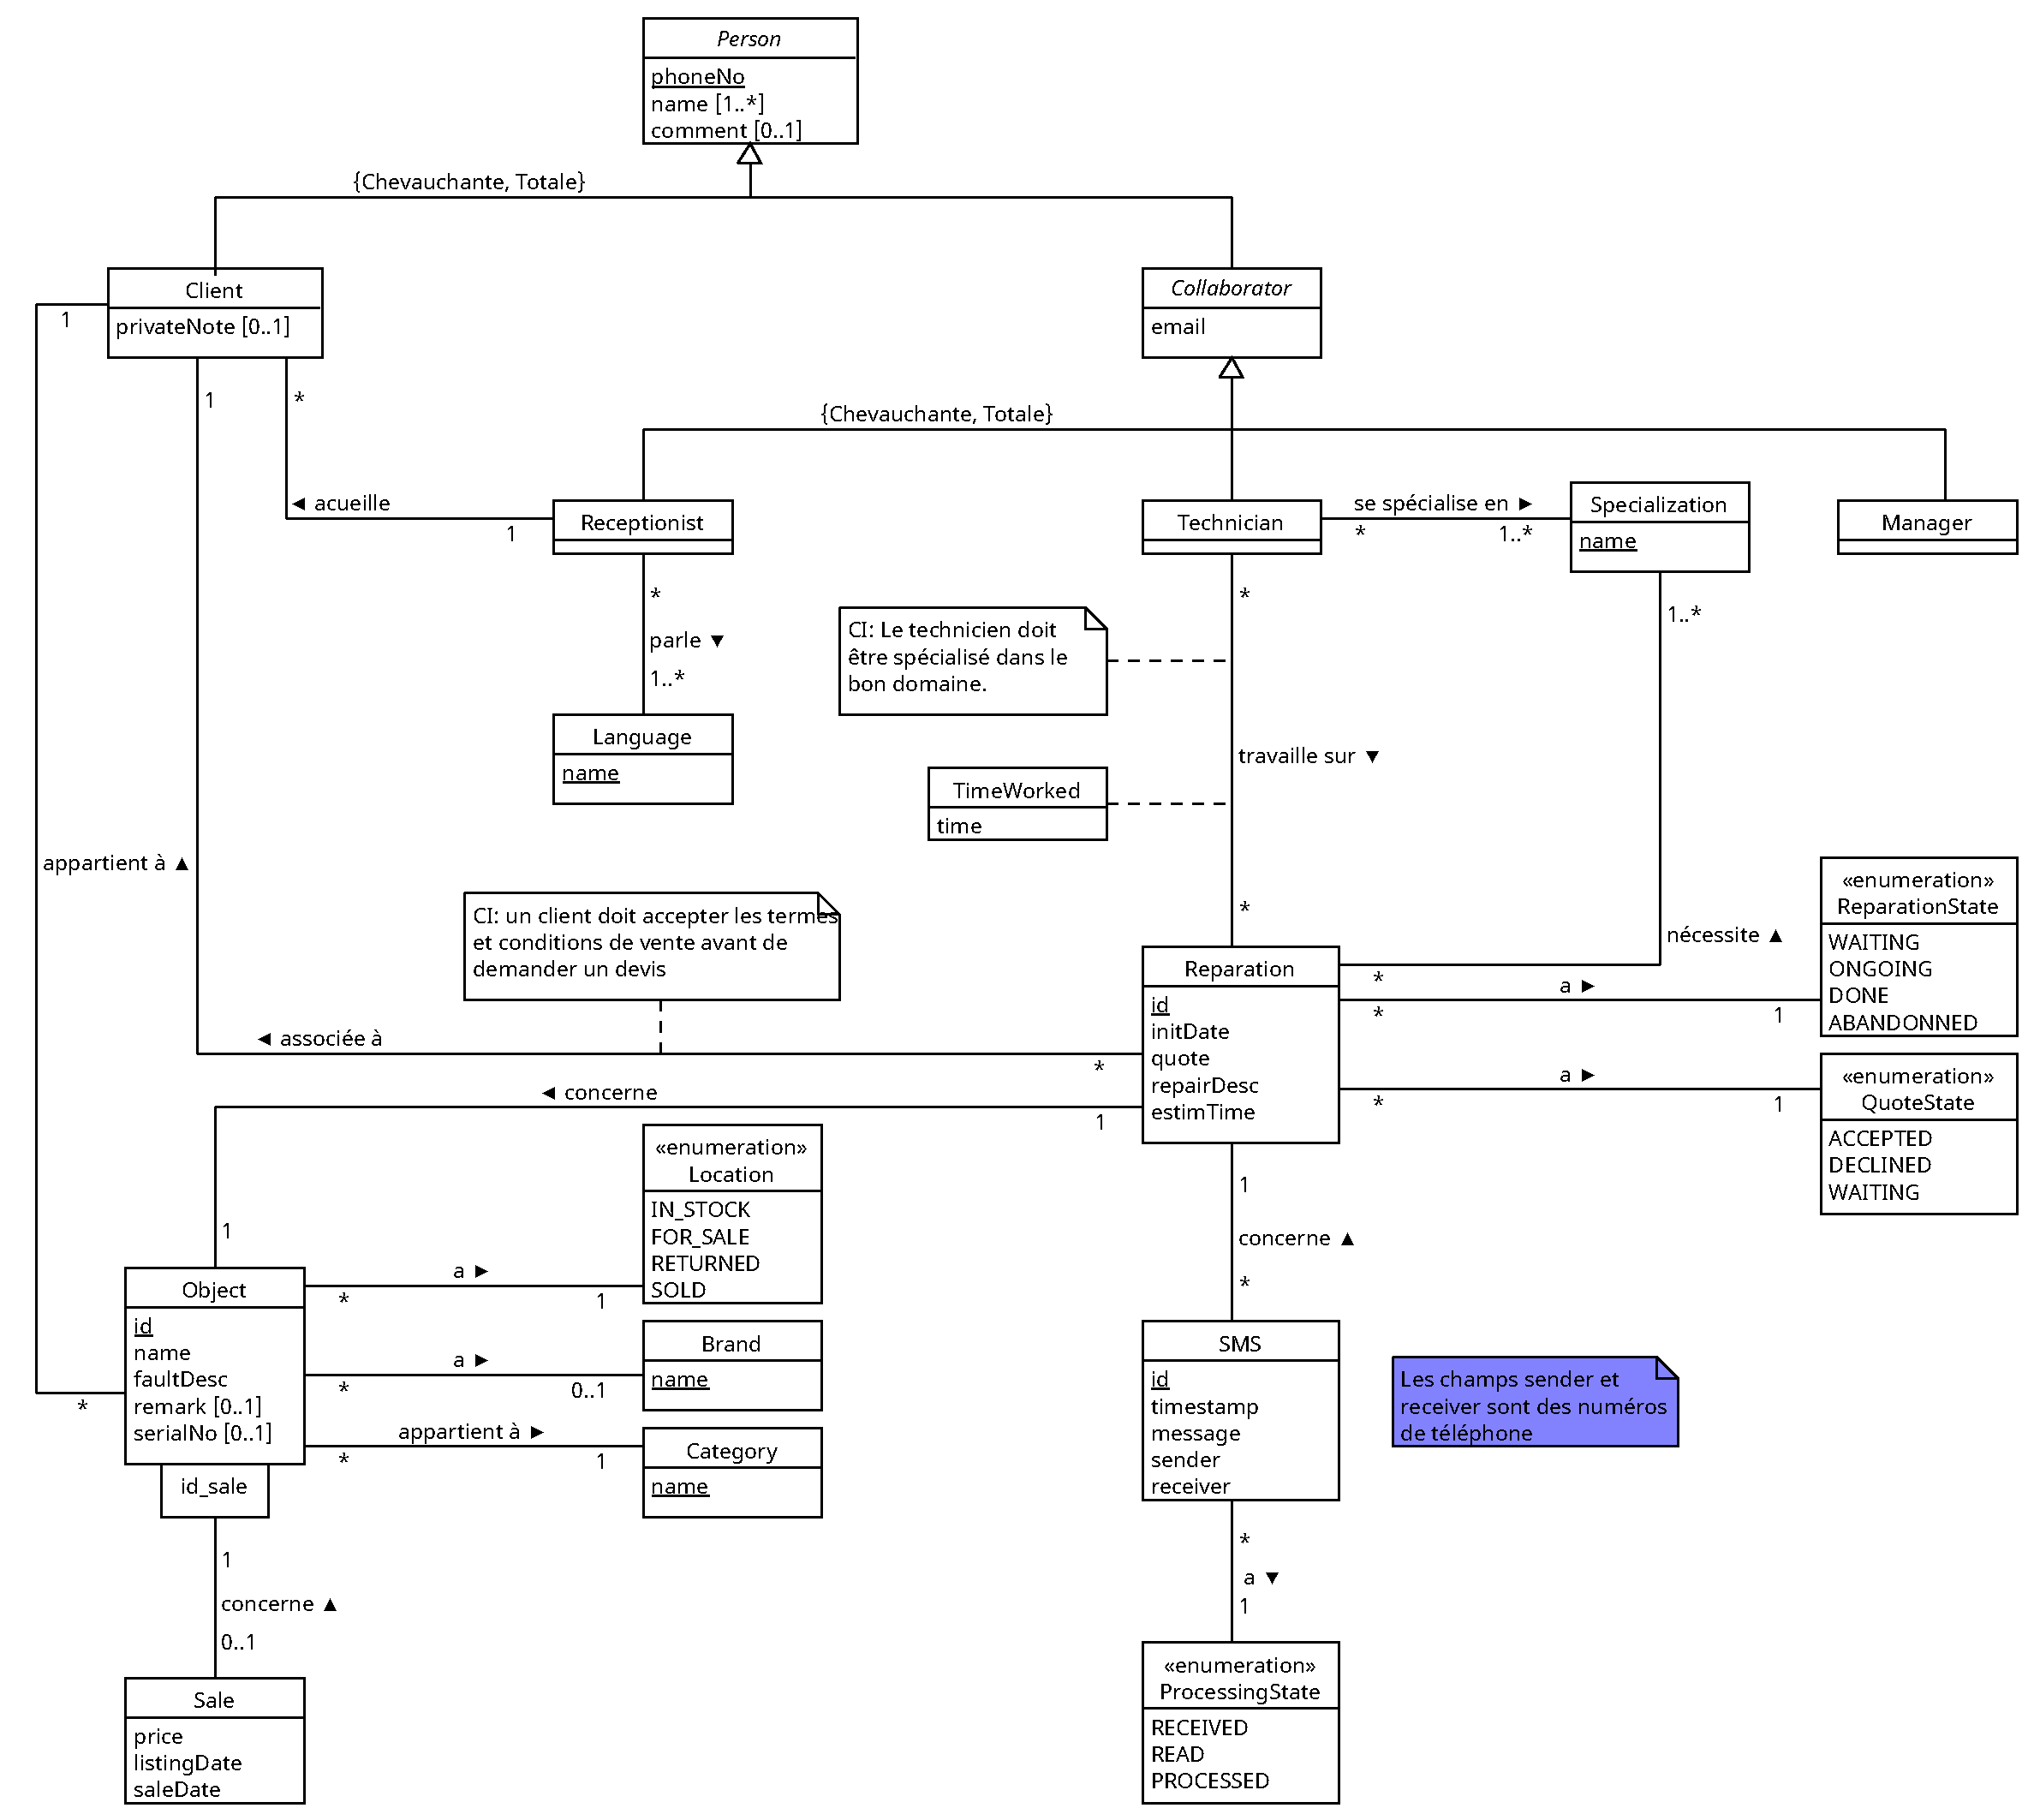
\includegraphics[height=0.93\textheight]{../assets/uml.pdf}
%         \caption{Schéma relationnel de la base de données.}
% \end{figure}
% \end{landscape}

\end{document}
